% !TeX TXS-program:compile = txs:///lualatex/[--shell-escape]
\documentclass[a4paper,14pt,russian]{extreport}

\usepackage[english,main=russian]{babel}

%\usepackage{newtxmath}
\usepackage[no-math]{fontspec}
\usepackage{polyglossia}

\defaultfontfeatures{Ligatures = TeX, Mapping = tex-text}

\setmainlanguage[babelshorthands = true]{russian}
\setotherlanguage{english}

\setmainfont{Times New Roman}

\newfontfamily\cyrillicfont{Times New Roman}
\newfontfamily\englishfont{Times New Roman}

\usepackage[
	left=30mm,
	right=10mm, 
	top=20mm,
	bottom=20mm,
]{geometry}

\makeatletter
	\renewcommand\LARGE{\@setfontsize\LARGE{22pt}{20}}
	\renewcommand\Large{\@setfontsize\Large{20pt}{20}}
	\renewcommand\large{\@setfontsize\large{16pt}{20}}
\makeatother

\usepackage{microtype} % Настройка переносов
\sloppy

\usepackage{setspace} % Настройка межстрочного интервала
\onehalfspacing

\usepackage{indentfirst} % Настройка абзацного отступа
\setlength{\parindent}{12.6mm}

\usepackage[unicode,hidelinks]{hyperref}
\usepackage{xifthen}

\usepackage{colortbl}

\usepackage[normalem]{ulem}
% Текст под линией 
\newcommand*{\undertext}[2]{%
	\begin{tabular}[t]{@{}c@{}}%
		#1\\\relax\scriptsize(#2)%
	\end{tabular}
}

% горизонтальная линия
\makeatletter
\newcommand{\vhrulefill}[1]
{
	\leavevmode\leaders\hrule\@height#1\hfill \kern\z@
}

\usepackage[figure,table]{totalcount} % Подсчет изображений, таблиц
\usepackage{rotating} % Поворот изображения вместе с названием
\usepackage{lastpage} % Для подсчета числа страниц

\usepackage{titlesec}
\usepackage{titletoc}
\usepackage{tocloft}

\setcounter{tocdepth}{5}

\setlength{\cftbeforetoctitleskip}{-25pt}
\renewcommand{\cfttoctitlefont}{\large\bfseries}

\renewcommand{\cftchapfont}{\large\bfseries}
\renewcommand{\cftsecfont}{\large}
\renewcommand{\cftchapleader}{\cftdotfill{\cftdotsep}}

\setlength{\cftbeforepartskip}{10pt}


\setcounter{secnumdepth}{5}

\titleformat{\part}[block]
{\large\bfseries}{\thechapter}{0.5em}{\large\centering}

\titleformat{\chapter}[block]
% {\large\bfseries}{\thechapter}{0.5em}{\large\raggedright}
{\hspace{\parindent}\large\bfseries}{\thechapter}{0.5em}{\large\raggedright}

\titleformat{\section}[block]
% {\large\bfseries}{\thesection}{0.5em}{\large\raggedright}
{\hspace{\parindent}\large\bfseries}{\thesection}{0.5em}{\large\raggedright}
\renewcommand{\thesection}{\arabic{chapter}.\arabic{section}.}

\titleformat{\subsection}[block]
{\hspace{\parindent}\large\bfseries}{\thesubsection}{0.5em}{\large\raggedright}
\renewcommand{\thesubsection}{\arabic{chapter}.\arabic{section}.\arabic{subsection}.}

\titleformat{\subsubsection}[block]
{\hspace{\parindent}\large\bfseries}{\thesubsubsection}{0.5em}{\large\raggedright}
\renewcommand{\thesubsubsection}{\arabic{chapter}.\arabic{section}.\arabic{subsection}.\arabic{subsubsection}.}

\titleclass{\part}{top}
\titlespacing*{\part}{12.5mm}{-22pt}{10pt}

\titlespacing{\chapter}{12.5mm}{-22pt}{10pt}
\titlespacing{\section}{12.5mm}{10pt}{10pt}
\titlespacing{\subsection}{12.5mm}{10pt}{10pt}
\titlespacing{\subsubsection}{12.5mm}{10pt}{10pt}

% ---------------------------------------- CAPTION --------------------------------- %

\usepackage[
	labelsep=endash,
	singlelinecheck=false,
]{caption}

\captionsetup[figure]{justification=centering}
\captionsetup[table]{justification=raggedleft}
\captionsetup[listing]{justification=raggedright}
\usepackage{caption} %заголовки плавающих объектов

\captionsetup[figure]{name=Рисунок}


% ---------------------------------------- ABBRS --------------------------------- %

\usepackage{enumitem}
\newcounter{descriptcount}
\newlist{enumdescript}{description}{2}
\setlist[enumdescript,1]{%
	before={\setcounter{descriptcount}{0}%
		\renewcommand*\thedescriptcount{\arabic{descriptcount})}}
	,font=\stepcounter{descriptcount}\thedescriptcount~
}
\setlist[enumdescript,2]{%
	before={\setcounter{descriptcount}{0}%
		\renewcommand*\thedescriptcount{\roman{descriptcount}}}
	,font=\stepcounter{descriptcount}\thedescriptcount~
}

\def\labelitemi{--} % Изменение буллета для списков


% ---------------------------------------- TABLE  ----------------------------------------

\usepackage{xcolor}
\usepackage{tabularx}
\usepackage{booktabs}
\usepackage{multirow}

\newcolumntype{O}{>{\centering\arraybackslash}p{0.08\textwidth}}
\newcolumntype{T}{>{\centering\arraybackslash}p{0.3\textwidth}}
\newcolumntype{L}{>{\centering\arraybackslash}p{0.45\textwidth}}
\newcolumntype{P}{>{\centering\arraybackslash}p{0.2\textwidth}}
\newcolumntype{R}{>{\centering\arraybackslash}p{0.22\textwidth}}
\newcolumntype{F}{>{\centering\arraybackslash}p{0.25\textwidth}}
\newcolumntype{S}{>{\centering\arraybackslash}p{0.15\textwidth}}
\newcolumntype{U}{>{\centering\arraybackslash}p{0.16\textwidth}}
\newcolumntype{N}{>{\centering\arraybackslash}p{0.19\textwidth}}
\newcolumntype{H}{>{\centering\arraybackslash}p{0.13\textwidth}}
\newcolumntype{E}{>{\centering\arraybackslash}p{0.18\textwidth}}
\newcolumntype{G}{>{\centering\arraybackslash}p{0.6\textwidth}}
\newcolumntype{Q}{>{\centering\arraybackslash}p{0.1\textwidth}}

% ---------------------------------------- FIGURE ----------------------------------------

\usepackage{graphicx}
\usepackage{float}
\usepackage{wrapfig}
\usepackage{tikzscale}
\usepackage[notransparent]{svg}
\svgpath{{assets/}}
\makeatletter
	\let\quote@name\unquote@name
\makeatother


\usepackage{pgfplots}
\pgfplotsset{compat=newest}

% ----------------------------------------- MATH -----------------------------------------

\usepackage{lscape}
\usepackage{afterpage}

\usepackage{amsmath}

\DeclareMathOperator*{\argmax}{arg\,max}
\DeclareMathOperator*{\argmin}{arg\,min}
% ----------------------------------------- LST -----------------------------------------
\usepackage{listings}
\usepackage{courier}

%\usepackage[cache=false, newfloat]{minted}
%\newenvironment{code}{\captionsetup{type=listing}}{}
\renewcommand{\lstlistingname}{Листинг}

\newcommand{\codefont}{\fontfamily{pcr}}
\newcommand{\keywordsfont}{\fontfamily{pcr}\bfseries}

%\usepackage{listings-golang} % import this package after listings
%\usepackage{minted}
% \lstset{
% 	basicstyle=\codefont\footnotesize,
% 	keywordstyle=\keywordsfont\color{black},
% 	numbers=left,
% 	numberstyle=\fontfamily{pcr}\tiny,
% 	showstringspaces=false,
% 	numbersep=10pt,
% 	tabsize=4,
% 	frame=tblr,	
% 	xleftmargin=25pt,
% 	framexleftmargin=18pt,
% 	framexrightmargin=-5pt,
% %	framexbottommargin=10pt,
% %	linewidth=0.95\pagewidth
% }

\usepackage[ruled,linesnumbered,resetcount,algochapter]{algorithm2e}
\SetKwInput{KwData}{Исходные параметры}
\SetKwInput{KwResult}{Результат}
\SetKwInput{KwIn}{Входные данные}
\SetKwInput{KwOut}{Выходные данные}
\SetKwIF{If}{ElseIf}{Else}{если}{тогда}{иначе если}{иначе}{конец условия}
\SetKwFor{While}{до тех пор, пока}{выполнять}{конец цикла}
\SetKw{KwTo}{от}
\SetKw{KwRet}{возвратить}
\SetKw{Return}{возвратить}
\SetKwBlock{Begin}{начало блока}{конец блока}
\SetKwSwitch{Switch}{Case}{Other}{Проверить значение}{и выполнить}{вариант}{в противном случае}{конец варианта}{конец проверки значений}
\SetKwFor{For}{цикл}{выполнять}{конец$\;$цикла} % очевидный и невероятный костыль
\SetKwFor{ForEach}{для каждого}{выполнять}{конец цикла}
\SetKwRepeat{Repeat}{повторять}{до тех пор, пока}
\SetAlgorithmName{Листинг}{алгоритм}{Список алгоритмов}

% ----------------------------------------- BIBLIO ---------------------------------------

\usepackage{totcount}
%\newtotcounter{citenum} %From the package documentation
%\AtEveryBibitem{\stepcounter{citenum}}

\usepackage[
	style=gost-numeric,
	language=auto,
	autolang=other,
	sorting=none,
	movenames=true,
	maxnames=3,
%	minnames=3,
	]{biblatex}
\usepackage{csquotes}

% Modify the @article style
\DeclareFieldFormat[article]{title}{#1} % Preserve the title as is

\newcounter{totalbibentries}
\newcommand*{\listcounted}{}

\makeatletter
\AtDataInput{%
	\xifinlist{\abx@field@entrykey}\listcounted
	{}
	{\stepcounter{totalbibentries}%
		\listxadd\listcounted{\abx@field@entrykey}}%
}
\makeatother


%\providecommand*{\BibDash}{}
\DeclareFieldFormat{extradate}{}

\DeclareFieldFormat[online]{title}{#1 [Электронный ресурс]}

\DeclareFieldFormat{urldate}{(дата обращения:\addspace\thefield{urlday}\adddot \thefield{urlmonth}\adddot\thefield{urlyear})}



\DeclareFieldFormat{url}{\bibstring{urlfrom}, URL:\addcolon\space\url{#1}}

\usepackage{url}
\urlstyle{same}

\usepackage{color} % Цвета для гиперссылок и листингов
\definecolor{comment}{rgb}{0,0.5,0}
\definecolor{plain}{rgb}{0.2,0.2,0.2}
\definecolor{string}{rgb}{0.91,0.45,0.32}
\hypersetup{citecolor=blue}
\hypersetup{citecolor=black}
\newfontfamily\lstfont{Times New Roman}
\usepackage{listings}
\lstset{
	basicstyle=\fontsize{14}{14}\linespread{1.0}\lstfont,
	language=python, % Или другой ваш язык -- см. документацию пакета
	commentstyle=\color{comment},
	numbers=left,
	numberstyle=\tiny,
	stepnumber=1,
	numbersep=5pt,
	xleftmargin =.19in,
	tabsize=4,
	extendedchars=\true,
	breaklines=true,
	keywordstyle=\color{black},
	frame=single,
	stringstyle=\lstfont\color{black}\lstfont,
	showspaces=false,
	showtabs=false,
	showstringspaces=false,
	showstringspaces=false,
	inputencoding=utf8x,
	keepspaces=true,
	captionpos=t,
	breakatwhitespace=false,
}
\DeclareCaptionFont{white}{\color{white}}
\captionsetup[lstlisting]{
	singlelinecheck=false,
	justification=centering,
	labelsep=endash,
}

\usepackage{color}
\usepackage[cache=false, newfloat]{minted}
\newenvironment{code}{\captionsetup{type=listing}}{}
\SetupFloatingEnvironment{listing}{name=Листинг}
\usepackage{float}
\usepackage{amsmath}

\usepackage{tocloft}

% Đặt căn lề trái cho các chương trong mục lục
\cftsetindents{chapter}{0cm}{2.5em}

% % Đặt căn lề trái cho các phần trong mục lục
\cftsetindents{part}{1.25cm}{2.5em}

% % Đặt căn lề trái cho các mục con (section) trong mục lục
\cftsetindents{section}{1cm}{2.5em}

% % Đặt căn lề trái cho các mục con con (subsection) trong mục lục
\cftsetindents{subsection}{1.27cm}{2.5em}
\addbibresource{biblio.bib}
\begin{document}
	%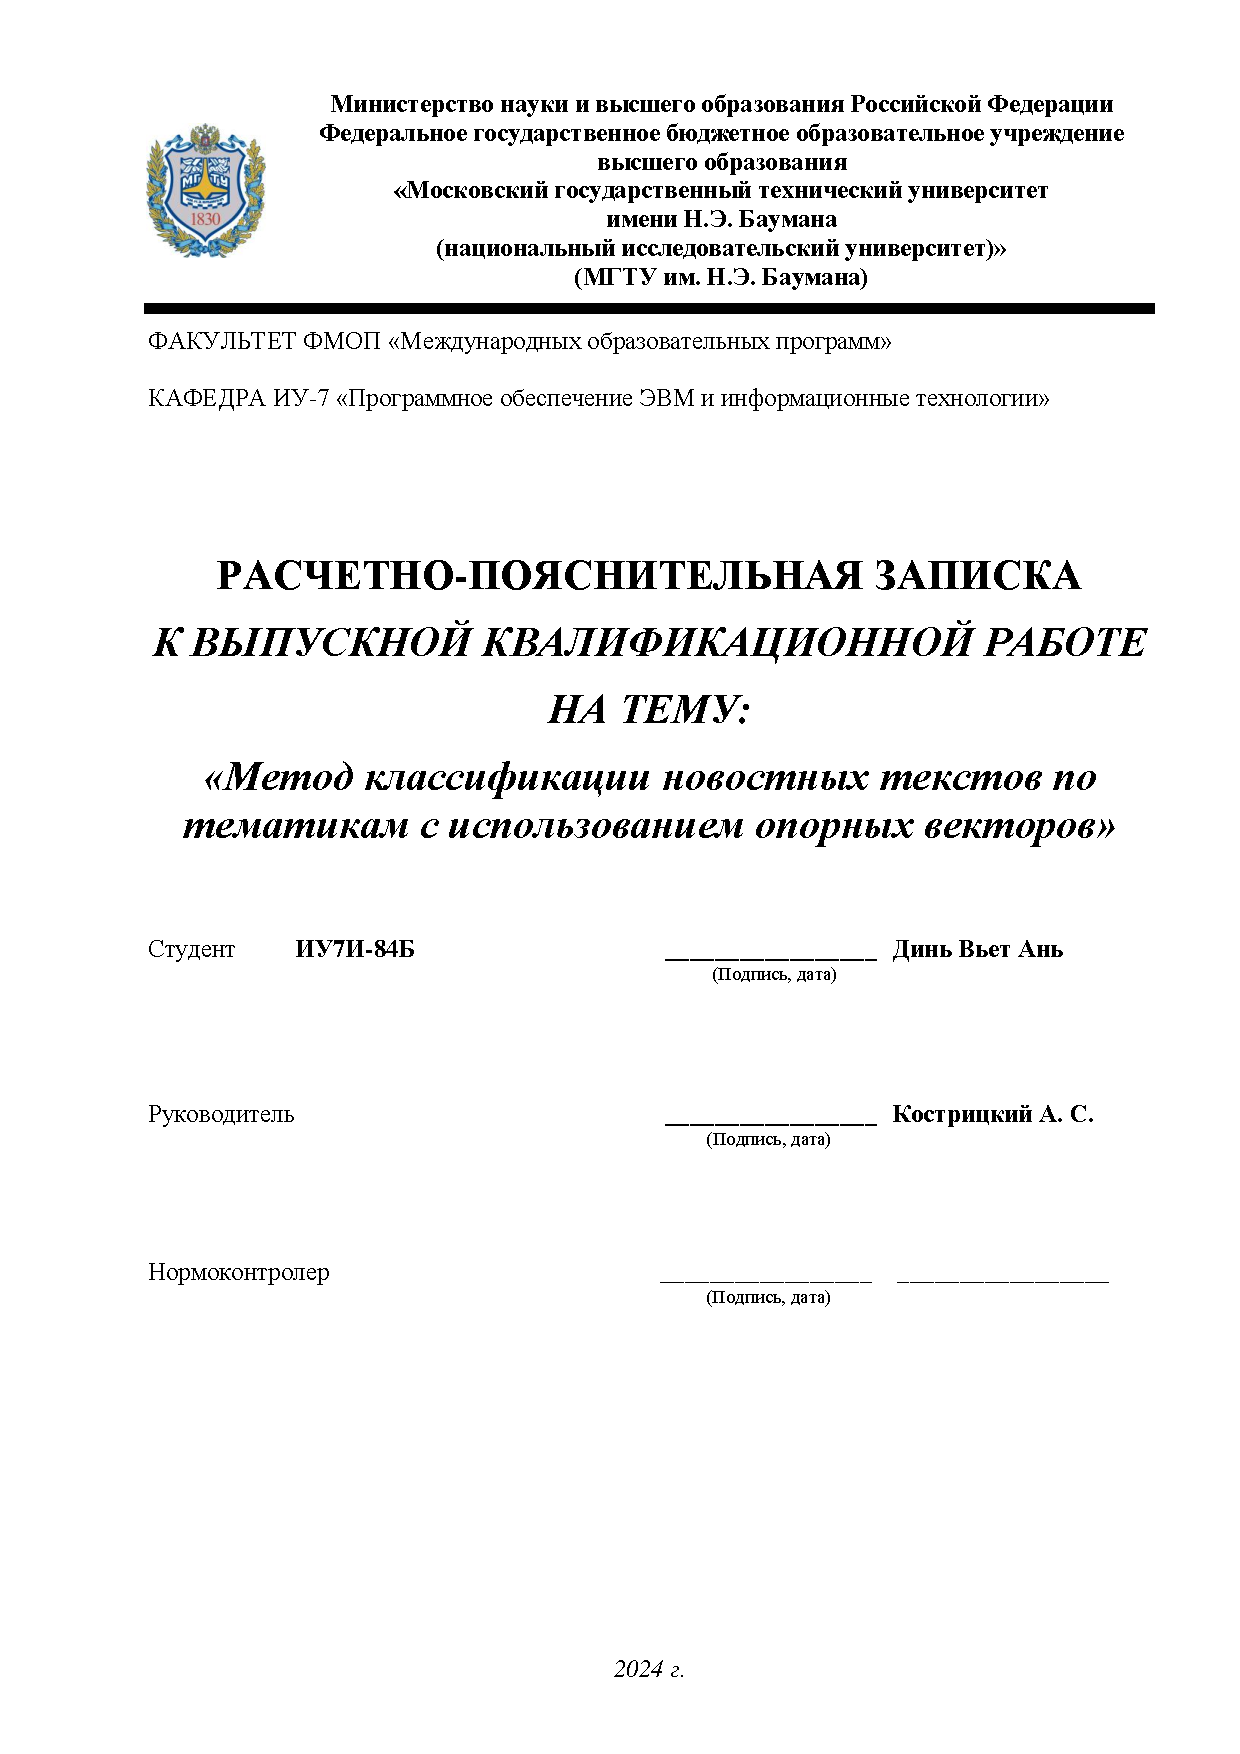
\includepdf{title.pdf}
	% \includepdf[pages=-]{calendar.pdf}
    % \the\cftsubsecindent
	\setcounter{page}{5}
	\part*{РЕФЕРАТ}
\addcontentsline{toc}{part}{РЕФЕРАТ}

Расчетно--пояснительная записка содержит 67 с., \totalfigures\ рис., \totaltables\ табл., 21 ист., 1 прил.

\textbf{Ключевые слова}: метод классификации, классификации текста, машинное обучение, метод опорных векторов.

В работе представлена разработка метода классификации новостных текстов по тематикам с использованием опорных векторов.

Рассмотрена задача классификации текста. Рассмотрены этапы решения задачи и основные методы классификации текста. Проведена формализация постановки задачи в виде IDEF0-диаграммы. Разработан метод классификации новостных текстов по тематикам с использованием опорных векторов. Представлена реализация разработанного метода, приведены результаты исследования качества классификатора в зависимости от различных параметров.

	\renewcommand{\contentsname}{\centerline{СОДЕРЖАНИЕ}} % Переименовать table of contents
    \tableofcontents


	\part*{ОПРЕДЕЛЕНИЯ, ОБОЗНАЧЕНИЯ И СОКРАЩЕНИЯ}
\addcontentsline{toc}{part}{ОПРЕДЕЛЕНИЯ, ОБОЗНАЧЕНИЯ И СОКРАЩЕНИЯ}
В настоящей расчетно-пояснительной записке применяют следующие термины с соответствующими определениям.
\begin{enumerate}
    \item SVM (англ. support vector machine) --- метод опорных векторов.
    \item KNN (англ. k-nearest neighbors) --- метод K-ближайших соседей.
    \item TF-IDF (англ. term frequency-inverse document frequency) --- Частота термина - обратная частота документа
\end{enumerate}
	\section*{ВВЕДЕНИЕ}
\addcontentsline{toc}{section}{ВВЕДЕНИЕ}

В последние годы наблюдается экспоненциальный рост количества сложных документов и текстов, требующих более глубокого понимания, чтобы иметь возможность точно классифицировать тексты во многих приложениях. Многие подходы к машинному обучению достигли превосходных результатов в обработке естественного языка. Успех этих методов зависит от их способности понимать сложные модели и нелинейные связи внутри данных. Однако поиск подходящих структур, архитектур и методов классификации текста является непростой задачей. 

Цель данной рабате --- проведение краткого обзора методов классификации текста, формулирование критерий оценки классификации текста и на их основе сравнить рассмотренных методов.

В рамках выполнения работы необходимо решить следующие задачи:

\begin{itemize}[label = ---]
    \item провести анализ предметной области;
    \item провести краткий обзор существующих методов классификации текста;
    \item сравнить рассмотренных методов по преимуществам и недостаткам.
\end{itemize}
	\chapter{Аналитический раздел}

В данном разделе приводятся анализ предметной области и этапы очистки и предварительной обработки текста, также рассматривается обзор методов извлечения признаков из текста. Также анализируются основные методы классификации текстов и проведено сравнение методов классификации текстов по преимуществам и недостаткам. Также в этом разделе представляется формализованная постановка задачи в виде IDEF0-диаграммы.

\section{Анализ предметной области}
\subsection{Задача классификации текстов}
Классификация текста —-- это процесс присвоения предопределенной категории или метки предложениям, абзацам, текстовым отчетам или неструктурированного текста.

За последние несколько десятилетий проблемы классификации текста широко изучались и решались во многих практических приложениях. Многие исследователи теперь заинтересованы в разработке приложений, использующих преимущества методов классификации текста, особенно в связи с недавними достижениями в области обработки естественного языка.

Некоторые задачи классификации текста в реальном \cite{task}:
\begin{enumerate}
    \item анализ настроений --- задача понимания аффективных состояний и субъективной информации, содержащейся в фрагменте текста;
    \item маркировка тем --- задача распознавания одной или нескольких тем фрагмента текста (т. е. его тем);
    \item классификация новостей --- задача присвоения новостям категорий;
    \item ответ на вопрос --- задача выбора ответа на вопрос, выбора из потенциальных предложений - кандидатов (обычно извлекаемых из контекстного документа);
    \item вывод на естественном языке --- задача определения того, влекут ли два предложения друг друга (классификация, происходит ли следование в одном из двух направлений или ни в одном из них);
    \item распознавание именованных объектов --- задача поиска именованных объектов в неструктурированном тексте и маркировка их заранее определенными категориями;
    \item синтаксический анализ --- серия задач, связанных с прогнозированием морфо - синтаксических свойств слов.
\end{enumerate}
\subsection{Процесс классификации текста}

Большинство процессов классификации текста, обычно, состоят из следующих трёх шагов: предобработка текста, извлечение признаков и классификации текста с помощью некоторого алгоритма. 

Ниже, на рисунке \ref{img:system}, представлены этапы процесса классификации текста.\newline
\captionsetup{justification=centering,singlelinecheck=off}
\begin{figure}[h!]
	\centering
		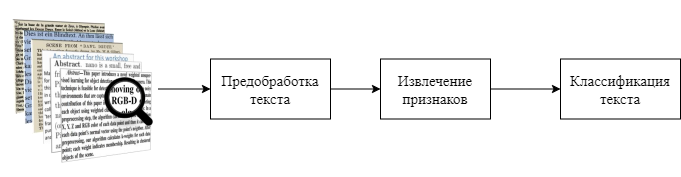
\includegraphics[,scale=0.7]{./img/system.png}
		\caption{Этапы процесса классификации текста.}  
		\label{img:system}
\end{figure}


Система классификации текстов содержит четыре различных уровня области применения, которые можно применять.
\begin{enumerate}
    \item Уровень документа. На этом уровне документа алгоритм получает соответствующие категории полного документа.
    \item Уровень абзаца. На этом уровне абзаца алгоритм получает соответствующие категории одного абзаца (части документа).
    \item Уровень предложения. На этом уровне предложения получают соответствующие категории одного предложения (части абзаца).
    \item Уровень подпредложения. На этом уровне подпредложения алгоритм получает соответствующие категории подвыражений внутри предложения.
\end{enumerate}
\section{Предобработка текста}
\subsection{Необходимость предобработки текста}

Входные данные для задач на естественном языке состоят из необработанного неструктурированного текста. Текстовая информация, в отличие от других типов данных, таких как изображения или временные ряды, не обладает числовым представлением, поэтому перед подачей ее в какой-либо классификатор она должна быть спроецирована в соответствующее пространство признаков. Поэтому процедуры предварительной обработки имеют особое значение, поскольку без них не существует основы ни для процедур выделения признаков, ни для алгоритмов классификации.

\subsection{Очистка и предобработка текста}
\textbf{Токенизация} --- самая базовая операция предварительной обработки, которую необходимо применить к тексту. Этот процесс определяет уровень детализации анализа текстовых данных и в целом может быть описан как процесс предварительной обработки, целью которого является разделение текстового потока на слова, фразы, символы или другие значимые элементы, называемые токенами. Разделение основано на правилах и может быть простым, как разделение пробелами или знаками препинания.

Например, предложение:

After eating, I decided to start working.

В данном случае токены следующие:

\{“After”, “eating”, “I”, “decided”, “to”, “start”, “working”\}.

\textbf{Стоп-слова} (текстовые шумы) —-- это неинформативные слова, которые встречаются в большом количестве, но не имеют семантического значения. Например, слова ``и'', ``в'', ``только'' не несут никакой ценности и только добавляют шум в данные. Множество токенов, полученный после процесса токенизации, может содержать множество ненужных или бессмысленных элементов. Удаление стоп-слов необходимо, поскольку это уменьшит количество различных элементов в пространстве признаков. 

Обычно тексты содержат разные грамматические формы одного и того же слова, а также могут встречаться однокоренные слова. Лемматизация и стемминг преследуют цель привести все встречающиеся словоформы к одной, нормальной словарной форме. 

\textbf{Стемминг} –-- это грубый эвристический процесс, который отрезает ``лишнее'' от корня слов, часто это приводит к потере словообразовательных суффиксов. 

\textbf{Лемматизация} –-- это более тонкий процесс, который использует словарь и морфологический анализ, чтобы в итоге привести слово к его канонической форме –-- лемме. 

Отличие в том, что стеммер (конкретная реализация алгоритма стемминга) действует без учёта контекста и, соответственно, не делает разницы между словами, которые имеют разный смысл в зависимости от части речи. Однако у стеммеров есть своё преимущество –-- они работают быстрее.
\section{Извлечения признаков}
\subsection{Модель Bag of Words}
\textbf{Модель Bag of Words} (модель BoW)\cite{phan1} —-- это уменьшенное и упрощенное представление текстового документа из выбранных частей текста на основе определенных критериев, таких как частота слов.

При всей простоте реализации данный подход имеет ряд недостатков:

\begin{itemize}[label = ---]
    \item для больших наборов текстов размерность словаря, а, следовательно, и размерность вектора, представляющего текст, может исчисляться сотнями тысяч, а иногда и миллионами;
    \item не учитывается контекст слова в документе.
\end{itemize}
\subsection{Метод Word2Vec}
\textbf{Word2Vec} (Word to Vector)\cite{phan1} —-- это метод, используемый для преобразования слов в векторы, тем самым фиксируя их значение, семантическое сходство и взаимосвязь с окружающим текстом. Этот метод помогает компьютерам изучать контекст и значение выражений и ключевых слов из больших текстовых коллекций, таких как новостные статьи и книги.

Основная идея Word2Vec состоит в том, чтобы представить каждое слово как многомерный вектор, где положение вектора в этом многомерном пространстве отражает значение слова.

Word2Vec использует модель мелкой нейронной сети для изучения значения слов из большого массива текстов. В отличие от глубоких нейронных сетей, которые имеют несколько скрытых слоев, мелкие нейронные сети имеют только один или два скрытых слоя между входом и выходом. Это делает обработку быстрой и прозрачной. Неглубокая нейронная сеть Word2Vec может быстро распознавать семантические сходства и идентифицировать слова-синонимы, что делает ее быстрее глубоких нейронных сетей.
\subsection{Алгоритм GloVe}
\textbf{GloVe} (Global Vector)\cite{phan1} --- алгоритм обучения без учителя  для получения векторных представлений слов. Обучение проводится на основе агрегированной глобальной статистики частоты совпадения слов из корпуса, и полученные представления демонстрируют интересные линейные подструктуры векторного пространства слов.  

Преимущества GloVe:
\begin{itemize}[label = ---]
    \item простая архитектура без нейронной сети;
    \item модель быстрая, и этого может быть достаточно для простых приложений;
    \item GloVe улучшает Word2Vec. Она добавляет частоту встречаемости слов и опережает Word2Vec в большинстве приложений;
    \item осмысленные эмбеддинги.
\end{itemize}

Недостатки алгоритма:
\begin{itemize}[label = ---]
    \item хотя матрица совместной встречаемости предоставляет глобальную информацию, GloVe остаётся обученной на уровне слов и даёт немного данных о предложении и контексте, в котором слово используется;
    \item плохо обрабатывает неизвестные и редкие слова.
\end{itemize}
\subsection{FastText}
\textbf{FastText}\cite{phan1} —-- это созданная в Facebook библиотека, содержащая предобученные готовые векторные представления слов и классификатор, то есть алгоритм машинного обучения разбивающий тексты на классы.

К основной модели Word2Vec добавлена модель символьных n-грамм. Каждое слово представляется композицией нескольких последовательностей символов определённой длины. Например, слово they в зависимости от гиперпараметров, может состоять из “th”, “he”, “ey”, “the”, “hey”. По сути, вектор слова – это сумма всех его n-грамм.

Результаты работы классификатора хорошо подходят для слов с небольшой частотой встречаемости, так как они разделяются на n-граммы. В отличие от Word2Vec и Glove, модель способна генерировать эмбеддинги для неизвестных слов.
\subsection{TF-IDF}
\textbf{TF-IDF} (англ. term frequency-inverse document frequency) --- статистическая мера, используемая для
оценки важности слова в контексте документа. Большой вес в TF-IDF получают слова с высокой частотой в пределах конкретного документа и с низкой частотой употребления в других документах. Вычисление вес в TF-IDF состоит из трех этапов. Первым этапом выполняется подсчет доли вхождений каждого слова (TF) по формуле (\ref{eq:TF}).
\begin{equation}\label{eq:TF}
	TF(word) = \frac{W(word)}{A},
\end{equation}
где W(word) --- количество вхождений слова word в документ, A --- количество всех слов в документе.

Вторым этапом выполняется измерение того, насколько важно это слово (IDF) по формуле (\ref{eq:IDF}).
\begin{equation}\label{eq:IDF}
    IDF(word) = \log\frac{D}{DW(word)} ,
\end{equation}
где D --- общее количество документов, DW(word) --- количество документов, которые содержат слово word.

И третий этап совмещает первые две оценки.
\begin{equation}\label{eq:TFIDF}
    TF-IDF(word) = TF(word) \cdot IDF(word).
\end{equation}

TF-IDF предоставляет несколько ключевых преимуществ.
\begin{enumerate}
    \item Учет важности слов: TF-IDF учитывает как частоту слова в документе, так и его общую редкость по всей коллекции. Таким образом, он помогает выделять ключевые слова, которые часто встречаются в данном документе, но не слишком распространены в остальных.
    \item Устранение шума: Слова, которые встречаются в большинстве документов (стоп-слова), имеют низкий IDF и, следовательно, низкий общий вес TF-IDF. Это позволяет устранить шум и фокусироваться на более важных словах.
\end{enumerate}

\section{Основные методы классификации текстов}
\subsection{Логистическая регрессия}
При совместном обучении с учителями логистическая регрессия --- это выбор наилучших параметров для маркировки для получения эффективных результатов классификации. Логистическая регрессия похожа на линейную регрессию, поскольку нужно найти значения коэффициентов входных переменных. Разница декоммутируется в том, что выходные значения преобразуются с использованием нелинейных или логистических функций.

В зависимости от того, как вы обучаете свою модель, можно использовать оценки логистической регрессии для отображения вероятностей выборок, относящихся к классу 0 или 1. Это полезно, когда нужно повысить точность прогнозирования.

Как и в случае с линейной регрессией, логистическая регрессия лучше справляется со своей задачей, если вы удаляете ненужные аналогичные переменные. Модели логистической регрессии быстро усваиваются и подходят для задач двоичной классификации.

\subsection{Наивный байесовский классификатор}

Это вероятностный классификатор, обычно используемый в машинном обучении, но также может использоваться в качестве статистического метода. В основном он используется для предварительной обработки данных, поскольку его легко вычислить. Для прогнозирования целевого класса используются байесовское рассуждение и вероятностный вывод. Поскольку атрибуты играют важную роль в классификации, производительность может быть улучшена путем присвоения атрибутам различных весовых коэффициентов \cite{11}.

Производительность наивного байесовского классификатора зависит от точности оценки условной вероятности. Без достаточного количества обучающих данных трудно точно оценить эти условия. Поэтому для оценки условных вероятностей используются некоторые методы метаэвристики, такие как генетические алгоритмы и дифференциальная эволюция. В некоторых случаях преимущества этого классификатора ставятся под сомнение из-за условного предположения о независимости между атрибутами, которые влияют на эффективность классификации \cite{11}. Используются различные методы мета-обучения для повышения производительности, включая расширение структуры, выбор атрибутов, преобразование частоты, взвешивание атрибутов, взвешивание экземпляров и локальное обучение. Таким образом, наивный байесовский классификатор прост в реализации и в то же время эффективен с точки зрения надежности. Эти особенности делают классификаторы подходящими для решения задач обработки естественного языка.

\subsection{Метод опорных векторов}
Метод опорных векторов (англ. support vector machine, SVM) --- один из наиболее популярных методов обучения, который применяется для решения задач классификации, регрессии и обнаружения выбросов. Основная идея метода заключается в построении гиперплоскости, разделяющей объекты выборки оптимальным способом. В двумерном пространстве эту оптимальную гиперплоскость можно представить как линию, разделяющую пространство на две части: где одна часть пространства содержит точки данных, которые принадлежат одному классу, а другая часть пространства содержит точки данных, принадлежащие другому класс. Концепция линий, действующих как классификатор, верна только в том случае, если точки данных линейно разделимы. SVM также можно использовать для поиска оптимальной кривой, которая может использоваться для классификации точек данных, которые нельзя разделить линейно.


Преимущества метода:
\begin{itemize}[label = ---]
	\item хорошо работает с пространством признаков большего размера;
	\item метод находит разделяющую полосу максимальной ширины, позволяет в дальнейшем осуществлять более уверенную классификацию;
    \item метод использует подмножество обучающих точек в функции принятия решений (называемых опорными векторами), поэтому это также эффективно с точки зрения памяти.
\end{itemize}

Недостатки метода:
\begin{itemize}[label = ---]
	\item долгое время обучения (для больших наборов данных);
	\item неустойчивость к шуму: выбросы в исходных данных становятся опорными объектами-нарушителями и напрямую влияют на построение разделяющей гиперплоскости.
\end{itemize}

\subsection{Decision Tree and Random Forest}
Деревья решений (англ. Decision Tree) являются одними из самых ранних и популярных классификаторов\cite{45}. Структура этого метода представляет собой иерархическую декомпозицию пространства данных\cite{7}. Основная идея заключается в создании дерева на основе атрибута для категоризированных точек данных, но основная задача дерева решений заключается в том, какой атрибут или функция может находиться на родительском уровне, а какой должен быть на дочернем уровне\cite{161}.

Деревья решений работает в определенной последовательности, чтобы проверить соответствие решения определенному пороговому значению среди доступных значений. Тестирование выполняется в соответствии с определенными логическими правилами, аналогичными весам нейронной сети. На этапе роста дерева обучающий набор разбивается на части, а на этапе обрезки его данные суммируются. Деревья, основанные на ансамбле, используют методы расширения возможностей и упаковки для объединения нескольких классификаторов, которые используют разные правила принятия решений для разных наборов данных \cite{8}. Эти ансамбли показали выдающуюся производительность по сравнению с традиционными деревьями решений, но вычислительные затраты увеличиваются по мере добавления входных запросов \cite{8}.

Дерева решений обладают низкой эффективностью при обработке многомерных данных. Для решения этой проблемы предлагаются кластерные деревья. Инкрементные деревья принятия решений лучше всего подходят для потоков данных, поскольку они обладают способностью стабилизироваться в соответствии с накапливающимися данными. Они использует несколько атрибутов для обучаемых функций.

Ниже, на рисунке \ref{tree}, представлен принцип работы метода деревьев решений.
\captionsetup{justification=centering,singlelinecheck=off}
\begin{figure}[h!]
	\centering
		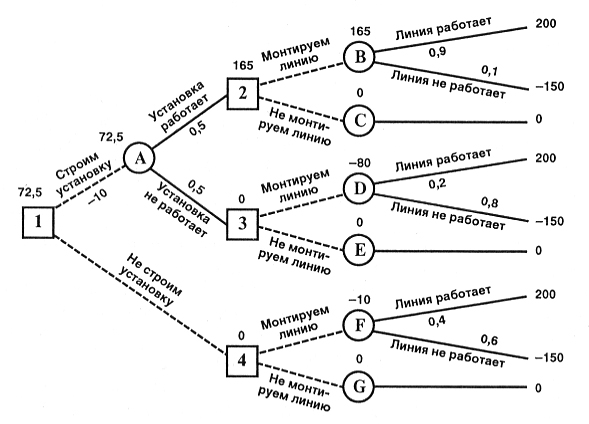
\includegraphics[,scale=1.3]{./img/decision_tree.png}
		\caption{Принцип работы метода деревьев решений}  
		\label{tree}
\end{figure}

Метод случайных лесов (Random Forest) --— это метод обучения для классификации текста. Случайные леса представляют собой наборы деревьев решений, обученных с использованием случайных подмножеств признаков, которые достигли гораздо более высокой производительности и чаще используются на практике. Этот метод очень быстро обучается работе с наборами текстовых данных по сравнению с другими методами, такими как глубокое обучение, но довольно медленным для создания прогнозов после обучения\cite{172}. Таким образом, чтобы добиться более быстрой структуры, количество деревьев в лесу необходимо уменьшить, поскольку большее количество деревьев в лесу увеличивает временную сложность на этапе прогнозирования.

\subsection{Метод K-ближайших соседей}
Метод K-ближайших соседей (англ. K-nearest neighbors, KNN) –-- это простой алгоритм машинного обучения с учителем, который можно использовать для решения задач классификации и регрессии.

Алгоритм K-NN сохраняет все доступные данные и классифицирует новую точку данных на основе сходства. Это означает, что когда появляются новые данные, их можно легко классифицировать по категории наборов с помощью алгоритма K-NN.

Согласно принципу алгоритма KNN, структура классификатора включает в себя 4 параметра: данные для классификации, набор выборочных данных, набор выборочных меток и значение K. Затем вычислить расстояние между новыми данными и выборочными данными, упорядочить расстояния от наименьшего к наибольшему, возьмите первые K ближайших данных. Наиболее часто встречающаяся метка может быть идентифицирована как новая метка данных путем определения количества вхождений каждого введенного типа данных в К первых точках.

Ниже, на рисунке \ref{knn}, представлен принцип работы метода K-ближайших соседей.
\captionsetup{justification=centering,singlelinecheck=off}
\begin{figure}[h!]
	\centering
		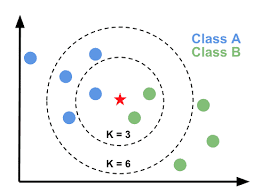
\includegraphics[,scale=1.0]{./img/knn.png}
		\caption{Принцип работы метода K-ближайших соседей}  
		\label{knn}
\end{figure}

Преимущества метода.
\begin{enumerate}
	\item Алгоритм прост и легко реализуем.
	\item Нет необходимости строить модель, настраивать несколько параметров или делать дополнительные допущения.
	\item Алгоритм универсален. Его можно использовать для обоих типов задач: классификации и регрессии.	
\end{enumerate}

Недостатки метода.
\begin{enumerate}
	\item Из аргумента выше следуют большие вычислительные затраты во время выполнения.
	\item Алгоритм работает медленнее при увеличении объема выборки.
	\item Всегда нужно определять оптимальное значение k.
\end{enumerate}

\subsection{Искусственные нейронные сети}
Искусственные нейронные сети (англ. Artificial Neural Network, ANN) имитируют работу человеческого мозга при принятии решений. Они работают, обучаются и развиваются с минимальным вмешательством человека или без него. Для классификации данных был предложен конкурентный алгоритм коэволюции, основанный на модели нейронной сети. Радиальные базовые функции являются компонентом ANN, поскольку они используют более быстрые алгоритмы обучения. Эта функция имеет компактную сетевую архитектуру, повышающую точность классификации. Кроме того, развив октябрьские алгоритмы, как правило, хорошо работают в динамических средах, адаптируются на лету и адаптируются к "нечетким" свойствам \cite{9}.

Нейронные сети также используются, когда требуется иерархический подход к классификации по нескольким тегам. Этот тип классификации означает, что каждая выборка может принадлежать более чем одному классу, и 1 уровень прогнозирования может использоваться в качестве входных данных для принятия окончательного решения на следующем уровне \cite{10}. 

ANN обладает отличной прикладной ценностью и потенциалом для разработки, а поскольку он не требует обучения отдельных бинарных классификаторов для задач с несколькими наборами, он создает лучший базовый классификатор с помощью подхода сообщества.

Сверточная нейронная сеть (англ. Convolutional neural network, CNN) —-- это архитектура глубокого обучения, которая обычно используется для иерархической классификации документов \cite{6}. Хотя CNN изначально были созданы для обработки изображений, они также эффективно использовались для классификации текста\cite{27}.

В базовой CNN для обработки изображений тензор изображения свернут с набором ядер размера d × d. Эти слои свертки называются картами объектов и могут объединяться для предоставления нескольких входных фильтров\cite{168}. Чтобы снизить сложность вычислений, CNN используют пуллинг для уменьшения размера выходных данных от одного уровня сети к другому. Различные методы объединения используются для уменьшения выходных данных при сохранении важных функций\cite{188}. Чтобы передать объединенные выходные данные составных избранных карт на следующий слой, карты сводятся в один столбец. Последние слои CNN обычно полностью связаны. В общем, на этапе обратного распространения ошибки сверточной нейронной сети корректируются как веса, так и фильтры детектора признаков. Потенциальная проблема, которая возникает при использовании CNN для классификации текста, это количество «каналов» S (размер пространства признаков). Хотя приложения классификации изображений обычно имеют мало каналов (например, только 3 канала RGB), S может быть очень большим (например, 50000) для приложений классификации текста, что приводит к очень высокой размерности\cite{187}. 

Было предложено множество подходов, одним из самых популярных является TextCNN\cite{69}, сравнительно простая модель на основе CNN с однослойной структурой свертки, которая размещается поверх вложений слов.

\section{Сравнение основные методов классификации текста}

Различные алгоритмы, обсуждавшиеся в этом разделе, суммированы в соответствии с их преимуществами и недостатками ниже, в таблице \ref{compare}.

\begin{table}[H]
	\centering
	\caption{Обзор различных методов классификации текста}\label{compare}
	\begin{tabular}{|m{7em}|m{12em}|m{12em}|}
		\hline
        \textit{Метод} & \textit{Преимущества} & \textit{Недостатки}\\ \hline
		Логистическая регрессия & Простая оценка параметров, хорошо работает для категориальных прогнозов & Требуется большой размер выборки, не подходит для нелинейных задач \\ \hline
  
        Наивный байесовский классификатор & Быстрый классификатор, требует меньшего времени обучения & Отсутствие взаимодействия между признаками \\ \hline
        
        Метод опорных векторов (SVM) & Эффективность в многомерных пространствах, простая реализация & Выбор наилучшего ядра, а также время, затраченное на обучение и тестирование \\ \hline
        
        Дерево решений & Простота интерпретации, легко визуализировать, быстрота обучения и прогнозирования & Чувствительность к шумам входных данных, сложен для неопределенных и многозначных атрибутов \\ \hline
        
        Метод К-ближайших соседей & Более простая реализация, гибкий выбор функций, хорошо подходит для много классовых задачи & Поиск ближайших соседей и оценка оптимального значения k \\ \hline
        Нейтронные сети & Простота использования, скорость реализации, приближены по возможностям к любым предыдущим алгоритмам & Требует больших обучающих и тестовых данных, большая часть операций скрыта и труднодоступна для повышения точности \\ \hline
	\end{tabular}
\end{table}

\section{Постановка задачи}
В настоящей работе проектируется метод классификации новостных текстов с помощью машинного обучения, а именно – метод опорных векторов. Набор данных для создания и обучения должен быть подготовлен для использования классификатором — а именно, должно быть установлено уникальное соответствие между новостным текстом и тематикой согласно разметке, представленной в наборе. Набор данных должен быть предварительно обработан и извлечены признаки. Обученный классификатор используется для распознавания тематика новостных текстов.

Ниже, на рисунке \ref{1-problem}, представлена IDEF0-диаграмма нулевого уровня.
\captionsetup{justification=centering,singlelinecheck=off}
\begin{figure}[h!]
	\centering
		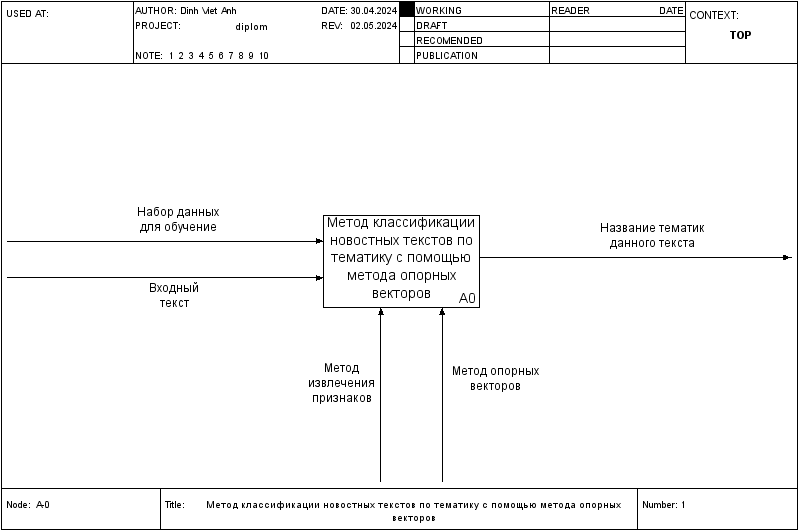
\includegraphics[,scale=0.55]{./img/01_A-0.png}
		\caption{IDEF0-диаграмма нулевого уровня}  
		\label{1-problem}
\end{figure}
\section*{Вывод}
В данном разделе был проведен анализ предметной области. Были рассмотрены методы очистки и предварительной обработки текста. Был проведен обзор методов извлечения признаков из текста. Был рассмотрены и проанализированы основные методы классификации текстов. Была представлена формализованная постановка задачи в виде IDEF0-диаграммы.

В разрабатываемом методе предлагается использовать подход, основанный на использовании TF-IDF для извлечения признаков, для классификации текстов использован метод опорных векторов.
	\chapter{Конструкторский раздел}
В этом разделе описывается этапы работы алгоритма разрабатываемого метода, также рассматриваются функциональные схемы обучения модели и метода классификации. Также приводятся метрики, используемые
для оценки качества работы обученной модели. Описывается используемый набор данных для обучения модели и рассматривается структура программного обеспечения.

\section{Структура программного обеспечения}

Разрабатываемый программный продукт состоит из следующих частей.
\begin{enumerate}
    \item Модуль предобработки текстов --- отвечает за очистку и предварительную обработку текстов.
    \item Модуль классификации --- отвечает за извлечение признаков из текстов, обучение модели и прогнозирование класса новых данных.
    \item Модуль создания выборки данных --- отвечает за создание файлов из скачанного набора данных.
    \item Модуль пользовательского интерфейса --- отвечает за предоставление пользовательского интерфейса.
\end{enumerate}

Внутри модуля предобработки текстов реализованы токенизация, удаление стоп-слов и лемматизация.

\section{Описание этапы работы алгоритма}
\subsection{Очистка и предобработка набора данных}

Прежде всего, набор данных необходимо очистить и предварительно обработать, поскольку это необходимый этап, как упоминалось в предыдущем разделе. Очистка текста включает в себя преобразование текста в нижний регистр, удаление лишних пробелов и небуквенно-цифровых символов.

Предобработка текстовых данных состоит из трех этапов: токенизация, удаление стоп-слов и лемматизация.

После токенизации исходный текст преобразуется в массив, элементами которого являются отдельные слова этого текста (токены). Текст будет сохранен как массив слов в том же порядке, что и в исходном тексте.

После удаления стоп-слов массив токенов уменьшит количество элементов, но не сильно повлияет на результат обучения модели, поскольку стоп-слова при удалении не потеряют смысла исходного текста.

После процесса лемматизация массив токенов будет преобразован в массив, элементы которого являются словами в их начальной форме с соответствующим типом слова.

\subsection{Формирование матрицы признаков}

Для извлечения признаков из массива токенов используется матрица признаков с помощью метода TF-IDF.

Сначала из массива слов будет создан список уникальных слов (словарь). На основе этого словаря рассчитывается значение IDF каждого слова в словаре. Затем для каждого текста в наборе данных рассчитывается вектор значений TF-IDF. Значения IDF и TF-IDF рассчитываются по формулам, рассмотренным в предыдущем разделе. Из векторов признаков создается матрица признаков, в которой каждая строка соответствует одному вектору признака одного текста после нормализация.

Каждый вектор признака нормализуется по формуле:

\begin{equation}
    \vec v_{norm} = \frac{\vec v}{\sqrt{\sum_{i=1}^n v_i^2}} = (\frac{v_1}{\sqrt{\sum_{i=1}^n v_i^2}}, \frac{v_2}{\sqrt{\sum_{i=1}^n v_i^2}}, ..., \frac{v_n}{\sqrt{\sum_{i=1}^n v_i^2}}),
\end{equation}
где $\vec v = (v_1, v_2, v_3, ..., v_n)$ --- вектор признака, $\sqrt{\sum_{i=1}^n v_i^2}$ --- длинна вектора $\vec v$, $\vec v_{norm}$ --- нормализованное вектор признака $\vec v$.

\subsection{Обучение классификатора}

Для выполнения классификации был выбран метод опорных векторов, потому что этот метод является одним из применимых алгоритмов машинного обучения, который используется для различных задач классификации и особенно подходит для данных большого размера\cite{svm21}. SVM --- линейный классификатор, основан на разделении множества векторов из n-мерного пространства гиперплоскостью. Этот метод требует обучения перед классификацией.

Поскольку в размеченном наборе данных есть несколько тематик, необходимо использовать многоклассовый классификатор. Для создания многоклассового классификатора используется подход "один против всех" (англ. one and rest). Этот подход заключается в подборе одного классификатора на класс. Для каждого классификатора класс сопоставляется со всеми другими классами. Таким образом, задачи многоклассовой классификации преобразуется в бинарную кластеризацию.

Основная идея метода заключается в построении гиперплоскости, разделяющей объекты выборки. То есть нужно найти гиперплоскость, которая задается следующим уравнением:
\begin{equation}
    (w, x) - b = 0,
\end{equation}
где $w$ --- вектор, $b$ --- число.

Тогда очевидно, что документы одного класса должны удовлетворять $(w, x_i) >= b$, а другого $(w, x_j) <= b$. Зафиксируем гиперплоскость, тогда параллельные гиперплоскости, содержащие опорные вектора, будут
выглядеть таким образом:
\begin{equation}
\begin{cases}
(w, x) = b + \epsilon, \\
(w, x) = b - \epsilon.
\end{cases}    
\end{equation}


Ниже, на рисунке \ref{svm1}, представлен принцип работы метода SVM.
\captionsetup{justification=centering,singlelinecheck=off}
\begin{figure}[h!]
	\centering
		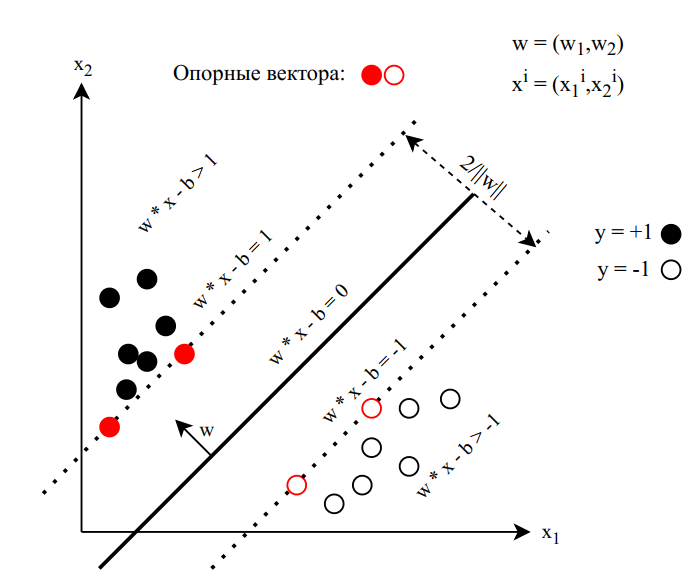
\includegraphics[,scale=0.8]{./img/svm1.png}
		\caption{Принцип работы метода опорных векторов}  
		\label{svm1}
\end{figure}
\newpage
Отклонение $\epsilon$ одно и тоже в силу того, что расстояние до опорных векторов будет одинаковым, иначе такая гиперплоскость точно не будет оптимальной.

После нормировки, а именно поделим вектор c и число d на $\epsilon$, получается:
\begin{equation}
\begin{cases}
(w', x) - b' = 1,\\
(w', x) - b' = -1.
\end{cases}
\end{equation}

Расстояние между двумя параллельными гиперплоскостями можно вычислить следующим образом:
\begin{equation}
    dist = \frac{|b_1 - b_2|}{||w||},
\end{equation}
где $b_1$ --- свободный член первой гиперплоскости, $b_2$ --- свободный член второй гиперплоскости, $||w|| = w \cdot w$ --- одинаков, вследствие параллельности гиперплоскостей.

Тогда несложно убедиться, что расстояние от параллельных гиперплоскостей до оптимальной гиперплоскости равно $\frac{1}{||w||}$. Теперь, чтобы найти оптимальную гиперплоскость, нужно решить следующую задачу оптимизации:
\begin{equation}
    \begin{cases}
    ||w|| \longrightarrow min, \\
    (w, x_i) - b \ge 1, \text{если }  y_i = 1, \\
    (w, x_j) - b \le -1, \text{если }  y_j = -1.
    \end{cases}
\end{equation}

Или в более удобной записи:
\begin{equation}
    \begin{cases}
    ||w|| \longrightarrow min, \\
    y_i \cdot [(w, x_i) - b] \ge 1, y_i \in \{-1; 1\}.
    \end{cases}
\end{equation}

Эта задача сводится к двойственной задаче поиска седловой точки функции Лагранжа. Но если в случае отсутствия линейной разделимости требуется ввести набор дополнительных переменных $\delta_i$, характеризующих величину ошибки на объектах $x_i \in \{x_1, ..., x_n\}$. Тогда задача оптимизации изменится следующим образом:

\begin{equation}
    \begin{cases}
    ||w|| + \sum\delta_i\longrightarrow min, \\
    y_i \cdot [(w, x_i) - b] \ge 1 - \delta_i, y_i \in \{-1; 1\}, \\
    \delta_i \ge 0, i \in \{1, ..., n\}.
    \end{cases}
\end{equation}

Здесь, $\delta_i$ равно нулю в том случае, если соответствующее неравенство выполняется и без него. То есть $\delta_i$ является минимально возможным значением, при котором неравенство будет выполнено. Решая эти задачи, можно получить вектор c, который и нужен для построения гиперплоскости.

Ниже, на рисунке \ref{svm2}, представлен вывод правил настройки весов.
\captionsetup{justification=centering,singlelinecheck=off}
\begin{figure}[h!]
	\centering
		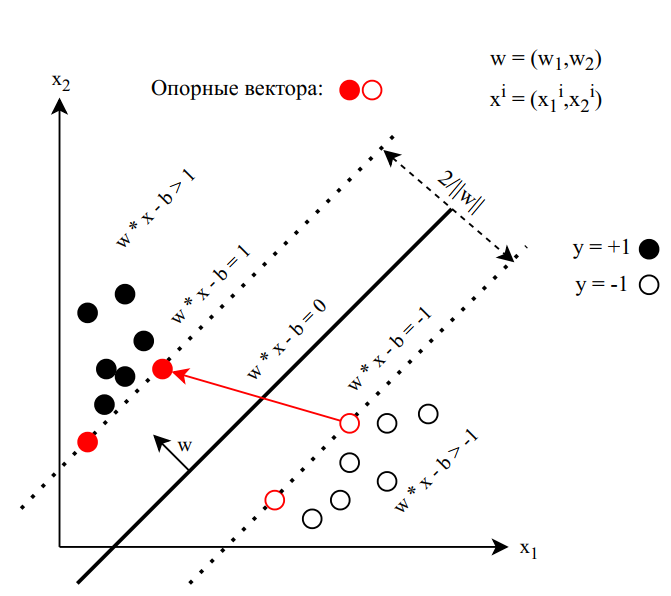
\includegraphics[,scale=0.8]{./img/svm2.png}
		\caption{Вывод правил настройки весов}  
		\label{svm2}
\end{figure}
\newpage
\subsection{Классификации текстов}

На данном этапе обученная модель получает на вход новостной текст. Этот текст необходимо очистить, предварительно обработать и извлечь признаки, используя те же этапы, что и для набора обучающих данных, чтобы получить соответствующие признаки. Входной текст преобразуется в вектор признаков и с помощью обученной модели прогнозирует тематику исходного новостного текста.

\section{Метрики оценки качества классификации текстов}

Показатели критериев оценки качества классификации, будут базироваться на следующих основных метриках результатов классификации на тестовой выборке.

\begin{itemize}[label = ---]
    \item TP (англ. True Positive) –-- истинный положительный результат. Верные данные, классифицированные как верные.
    \item TN (англ. True Negative) –-- истинный отрицательный результат. Неверные данные, классифицированные как неверные.
    \item FP (англ. False Positive) –-- ложный положительный результат. Верные данные, классифицированные как неверные.
    \item FN (англ. False Negative) –-- ложный отрицательный результат. Неверные данные, классифицированные как верные.
\end{itemize}

Для оценки качества модели, обученного на обучающей и тестовой выборках из набора данных, используются следующие две метрики: аккуратность и F1-мера.

Метрики аккуратности (англ. Accuracy) --- один из наиболее простых, а поэтому и распространенной метрикой. Она показывает количество правильно проставленных меток класса (суммы истинно положительных и истинно отрицательных результатов) от общего количества данных и считается следующим образом:
\begin{equation}
    Accuracy = \frac{TP + TN}{TP + TN + FP + FN}.
\end{equation}

F1-мера —-- это показатель оценки, который измеряет качество работы модели классификации. Он сочетает в себе оценки точности и полноты модели.

Точность модели (англ. Precision) —-- это показатель оценки модели и производительности, который соответствует доле значений, которые фактически принадлежат положительному классу, среди всех значений, которые, по прогнозам, принадлежат этому классу. Точность также известна как положительная прогностическая ценность (англ. positive predictive value, PPV). Оценка F1 использует точность, чтобы получить долю истинно положительных записей среди общего числа записей, классифицированных как положительные с помощью модели машинного обучения. Точность модели рассчитывается следующим образом:
\begin{equation}
    Precision = \frac{TP}{TP + FP}.
\end{equation}

Полноты модели (англ. Recall)--- это показатель оценки модели и производительности, который соответствует доле значений, которые, по прогнозам, относятся к положительному классу, среди всех значений, которые действительно принадлежат к положительному классу (включая ложно отрицательные). F1-мера использует полноты, чтобы получить долю истинно положительных записей среди общего числа фактически положительных записей. Полноты модели рассчитывается следующим образом:
\begin{equation}
    Recall = \frac{TP}{TP + FN}.
\end{equation}

Значение F1-меры рассчитывается как гармоническое среднее значений точности и полноты модели, по следующей формуле:
\begin{equation}
    F1 = 2 \cdot \frac{Precision \cdot Recall}{Precision + Recall} = \frac{TP}{TP + \frac{1}{2} (FP + FN)}.
\end{equation}

\section{Функциональная схема обучения модели}

Для обучения модели используется метод SVM, а для метода извлечения признаков из набора текстов используется метод TF-IDF. На входе поступает набор новостных текстов с соответствующей меткой для обучения, а на выходе --- обученная модель на этом наборе.

Ниже, на рисунке \ref{2-train} представлена функциональная схема обучения модели (с помощью SVM) в виде IDEF0-диаграммы. На этой схеме отображены этапы создания обучающей и тестовой выборок, очистки и предобработки текстов, извлечения признаков и выполнения многоклассовой классификации для обучающей
выборки.

\captionsetup{justification=centering,singlelinecheck=off}
\begin{figure}[h!]
	\centering
		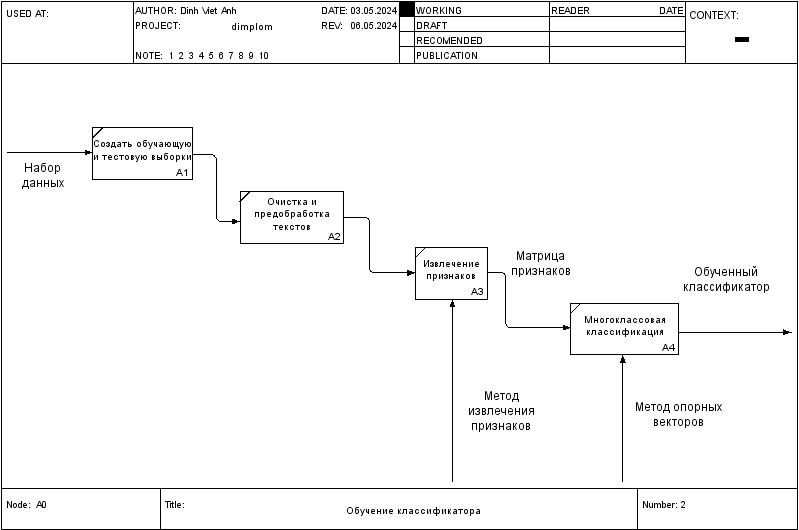
\includegraphics[,scale=0.55]{./img/train.png}
		\caption{Функциональная схема обучения модели}  
		\label{2-train}
\end{figure}
\newpage
\section{Функциональная схема метода классификации}

Ниже, на рисунке \ref{2-use} представлена функциональная схема метода классификации в виде IDEF0-диаграммы. На входе поступает новостной текст для классификации, а выходе --- прогнозируемое название тематика этого текста. 

На этой схеме отображены этапы очистки и предобработки входного текста, извлечения признаков и выполнения распознавания тематика текста, использующего обученную модель.

\captionsetup{justification=centering,singlelinecheck=off}
\begin{figure}[h!]
	\centering
		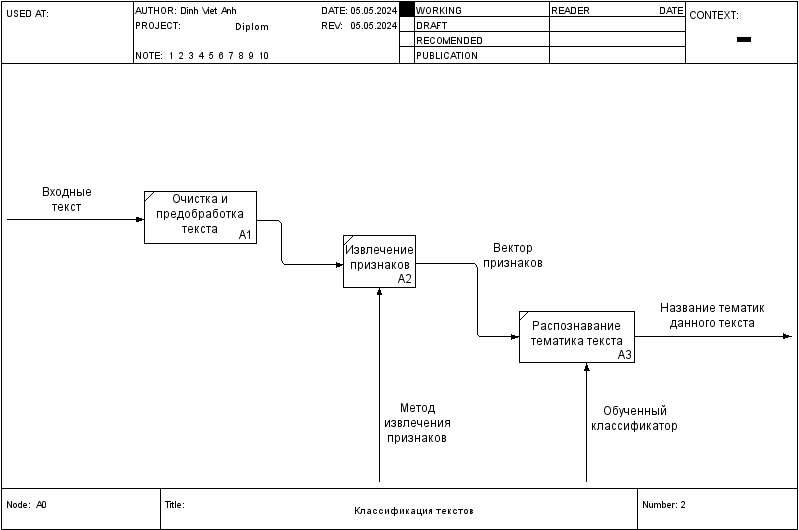
\includegraphics[,scale=0.55]{./img/use.png}
		\caption{Функциональная схема метода классификации}  
		\label{2-use}
\end{figure}
\newpage
\section{Описание используемого набора данных}

Для обучения модели было решено использовать набор данных News dataset from Lenta.Ru \cite{kaggle_data}. Этот набор данных содержит более 800 тысяч новостей на русском языке, соответствующих более чем 20 тематикам, с сентября 1999 года по декабрь 2019 года. Источник новостей —-- сайт lenta.ru \cite{lenta}, российское новостное интернет-издание, основанное в 1999 году. В наборе данных для каждой новости сохраняются текст, заголовок, тематик, дата публикации и ссылка на источник. Этот набор данных можно скачать с сайта Кaggle \cite{kaggle} --- система организации конкурсов по исследованию данных, а также социальная сеть специалистов по обработке данных и машинному обучению. 

После скачивания набора данных необходимо выполнить этап фильтрации данных, чтобы сохранить набор данных в виде файла CSV и создать наборы обучения для будущего использования.

Ниже, на рисунке \ref{2-file}, представлены примеры некоторых строк в наборе данных.

\captionsetup{justification=centering,singlelinecheck=off}
\begin{figure}[h!]
	\centering
		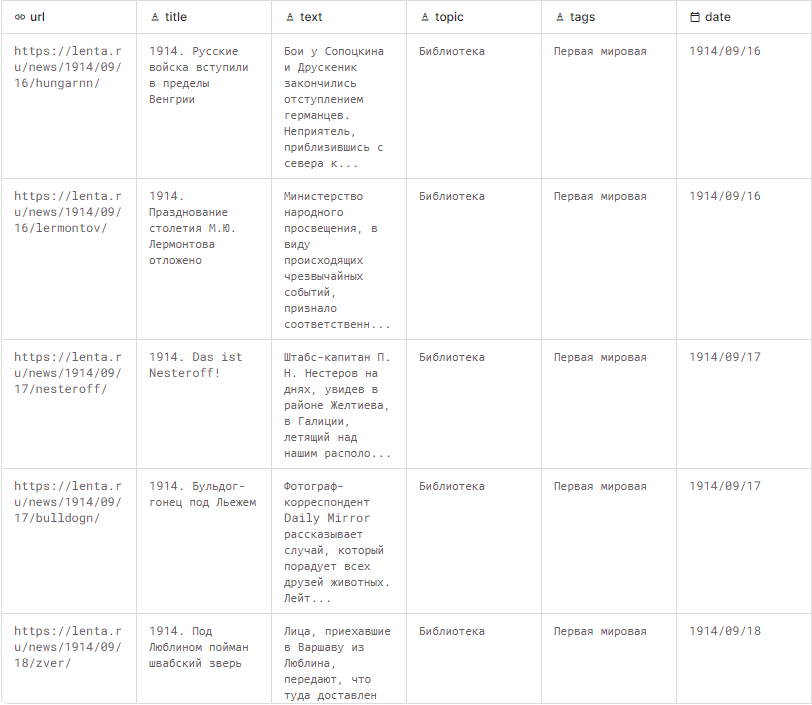
\includegraphics[,scale=0.75]{./img/file.png}
		\caption{Примеры некоторых строк в наборе данных}  
		\label{2-file}
\end{figure}
\newpage


\section*{Вывод}

В этом разделе были описаны этапы работы алгоритма разрабатываемого метода, также были рассмотрены функциональные схемы обучения модели и метод классификации. Также были приведены метрики, используемые для оценки качества работы обученного модели. Был описан используемый набор данных для обучения модели и была рассмотрена структура программного обеспечения.
	\chapter{Технологический раздел}
В этом разделе приводится выбор языка программирования и средства программирования и рассматриваются необходимые библиотеки, которые используются для разработки программного обеспечения. Также описывается формат входных и выходных данных. Также приводятся описание пользовательского интерфейса и руководство пользователя для установки и использования программного обеспечения.
\section{Выбор средств реализации программного обеспечения}
\subsection{Выбор языка программирования}
Для реализации программного обеспечения был использован язык программирования Python\cite{python}. Этот выбор обусловлен следующими причинами:
\begin{itemize}[label = ---]
    \item это язык программирования высокого уровня, имеет простой синтаксис;
    \item наличие библиотек с открытым исходным кодом, позволяющих работать с естественным языком, выпонять классификации методом SVM и визуализировать данные;
    \item имеется навыки использования данного языка программирования, что сократить время написания программы.
\end{itemize}

\subsection{Выбор среды программирования}
Для разработки программы использовалась среда Visual Studio Code \cite{vscode} в качестве среды разработки по следующим причинам:
\begin{itemize}[label = ---]
    \item доступна бесплатная версия;
    \item имеет множество утилит, упрощающих написание кода;
    \item имеется навыки программирования при помощью данной среды, что сократить время написания программы.
\end{itemize}

Библиотека scikit-learn используется для работы с машинным обучением, потому что она предоставляет множество различных инструментов для разных задач машинного обучения, включая кластеризацию, регрессию, кластеризацию, обучение и тестирование моделей, а также предварительную обработку данных, и так далее. 

Для создания пользовательского интерфейса используется фреймворк Qt c помощью библиотеки PyQt5. Кроме того, в процессе разработки программного обеспечения библиотека pandas также используется для анализа набора данных, а библиотеки nltk и pymorphy2 — для очистки и предварительной обработки текстов.

\section{Формат входных и выходных данных}
Для модуля создания выборки данных входными данными является набор данных, скачанный с сайта kaggle.com, а выходные данные представляют собой файлы с указанным количеством строк для каждой темы.

На этапе обучения модели входными данными является файл, который создается из набора новостных текстов, в формате файла CSV. Каждая строка соответствует новости, состоящему из двух частей: текста и тематика новости. Каждый файл содержит определенное количество текста по каждой тематику.

На этапе классификации входными данными является текст или текстовый файл (в формате файла TXT), содержащий текст. Текст должен быть на русском языке, не менее 10 слов.

Результатом модуля классификации является прогнозируемое название тематика входного текста или содержимого файла и выводятся на пользовательский интерфейс программного обеспечения.

\section{Руководство пользователя}

Для запуска разработанного программного обеспечения требуется установить интерпретатор для Python и используемые библиотеки. Используемые в разработке библиотеки, которые необходимы для запуска ПО, приведены в файле requirements.txt, который находится в корневом каталоге проекта. С помощью пакетного менеджера pip все зависимости можно установить или обновить, запустив в терминале команду, приведенную в листинге \ref{lst:library}.

\begin{lstlisting}[caption=Установка всех необходимых библиотек,label=lst:library]
pip install -r requirements.txt
\end{lstlisting}

Для работы библиотеки nltk необходимо скачать библиотеки. Для установки библиотеки nltk и скачивания библиотек нужно в коде программы выполнить команды, приведенные в листинге \ref{lst:nltk}

\begin{lstlisting}[caption=Установка словарей nltk, label=lst:nltk]
import nltk
nltk.download()
\end{lstlisting}

Для создания выборки необходимо разместить папку с файлом исходного набора данных внутри корневого каталога проекта и запустить скрипт dataset.py. Скрипт может запущен из графического интерфейса среды разработки, либо командой из терминала, приведенную в листинге \ref{lst:data}.

\begin{lstlisting}[caption= Команда для создания обучающих выборок, label=lst:data]
python dataset.py
\end{lstlisting}

Чтобы обучить модель на заранее созданных размеченных выборках и предсказать тематик входного текста или текстового файла, пользователь может воспользоваться графическим интерфейсом приложения. Для открытия приложения необходимо запустить скрипт main.py посредством интерфейса среды разработки или командой в терминале, приведенную в листинге \ref{lst:run}.

\begin{lstlisting}[caption=Команда для запуска приложения, label=lst:run]
python main.py
\end{lstlisting}

В результате разработанное программное обеспечение может установить тематик текста или выдвинуть предположение, что может быть тематикой.

\section{Интерфейс пользователя}
Пользовательский интерфейс, который представлен на рисунке \ref{1-program}, был разработан с помощью программы Qt Designer. Интеграция с кодом на Python осуществлена посредством с помощью библиотеки PyQt5, которая предоставляет различные классы для работы с объектами пользовательского интерфейса.

\captionsetup{justification=centering,singlelinecheck=off}
\begin{figure}[h!]
	\centering
		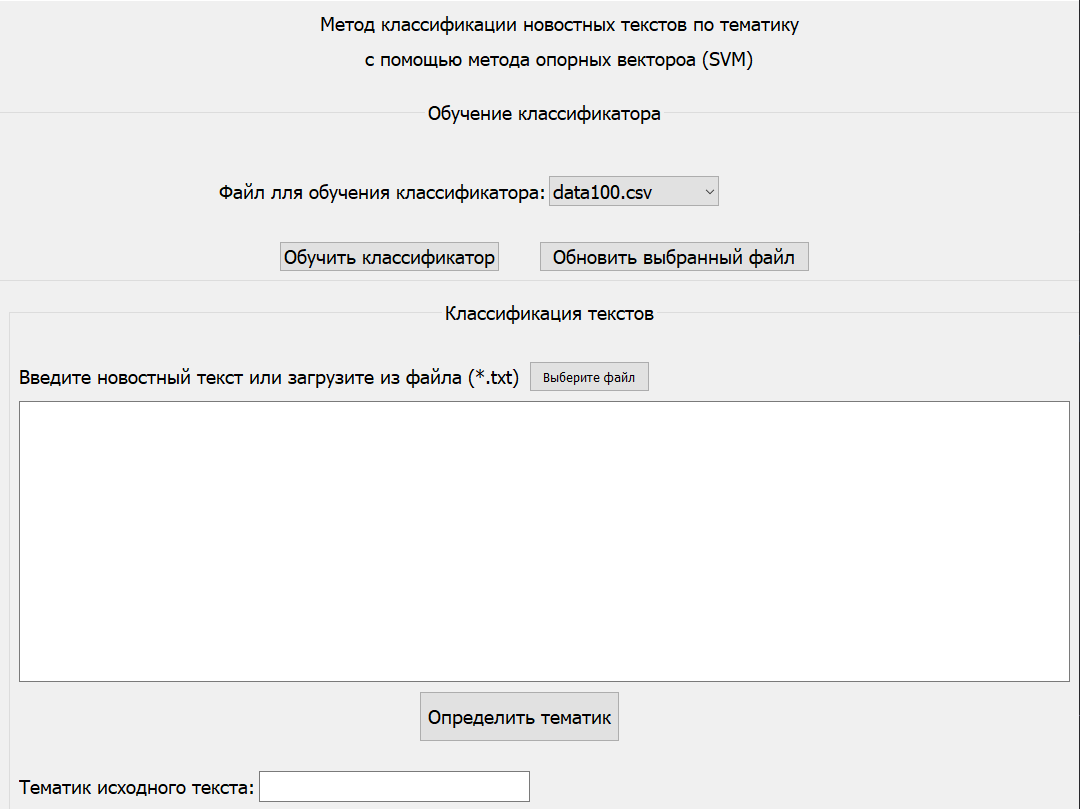
\includegraphics[,scale=0.55]{./img/1.png}
		\caption{Пользовательского интерфейса ПО}  
		\label{1-program}
\end{figure}
\newpage
Пользовательский интерфейс программного обеспечения состоит из 2 частей. В верхней части находится функционал обучения модели. В этом окне пользователь может выбрать файл для обучения модели из поля выбора. Каждый файл содержит определенное количество текста по каждой тематику. Пользователь может обновить содержимое этих файлов с помощью кнопки «Обновить выбранного файла». При нажатии на кнопку «Обучить модель» выбранная выборка разбивается на две части: 80\% корпуса –-- обучающая выборка, 20\% --– тестовая. Программа сообщит, когда модель завершит обучение , как показано на рисунке \ref{3-program}.

\captionsetup{justification=centering,singlelinecheck=off}
\begin{figure}[h!]
	\centering
		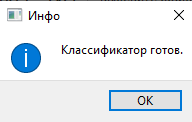
\includegraphics[,scale=1.5]{./img/3.png}
		\caption{Модель готова}  
		\label{3-program}
\end{figure}
\newpage
В нижней части находится функционал предсказания тематика текста. Если пользователь попытается определить тематик, не обучив сначала модель, будет возвращена ошибка, как показано на рисунке \ref{2-program}.

\captionsetup{justification=centering,singlelinecheck=off}
\begin{figure}[h!]
	\centering
		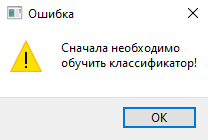
\includegraphics[,scale=1.55]{./img/2.png}
		\caption{Ошибка, возникающая в случае, если модель не обучена}  
		\label{2-program}
\end{figure}

Пользователь может ввести текст в поле ввода или выбрать файл. Программа поддерживает только txt файлы (текстовые файлы). При нажатии на кнопку «Выбрать файл» открывается файловая система компьютера, в которой необходимо выбрать интересующий текстовый файл. Когда пользователь выбирает файл, его содержимое отображается в текстовом поле. Если пользователь нажимает кнопку «Определить тематик», когда вводимый текст пуст или имеет неверный формат, будет возвращена ошибка, как показано на рисунке \ref{4-program}.

\captionsetup{justification=centering,singlelinecheck=off}
\begin{figure}[h!]
	\centering
		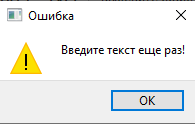
\includegraphics[,scale=1.5]{./img/4.png}
		\caption{Ошибка, возникающая в случае, если текстовое поле пусто}  
		\label{4-program}
\end{figure}
\newpage
Если входной текст не пуст, то запускается алгоритм классификации. После того, как модель завершит работать, на экран будет выведено название наиболее вероятного тематика, как показано на рисунке \ref{5-program}.

\captionsetup{justification=centering,singlelinecheck=off}
\begin{figure}[h!]
	\centering
		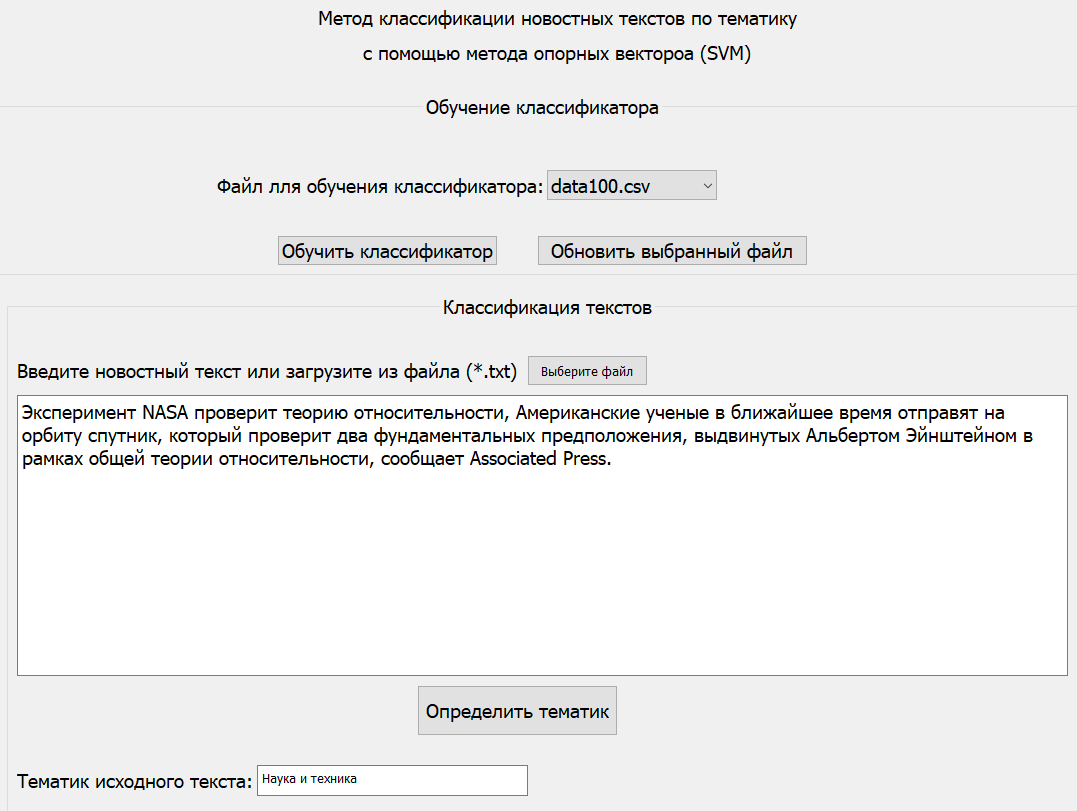
\includegraphics[,scale=0.55]{./img/5.png}
		\caption{Результат работы классификации}  
		\label{5-program}
\end{figure}

\section*{Вывод}
В этом разделе были приведены выбор языка программирования и средства программирования и рассмотрены необходимые библиотеки, которые используются для разработки программного обеспечения. Также был описан формат входных и выходных данных. Также были приведены описание пользовательского интерфейса и руководство пользователя для установки и использования программного обеспечения.
	\chapter{Исследовательский раздел}
\section{Технические характеристики}
Технические характеристики устройства, на котором выполнялись исследования разработанного метода:

\begin{itemize}
	\item[---] операционная система Window 10 Home Single Language \cite{window};
	\item[---] память 8 Гб;
	\item[---] процессор 11th Gen Intel(R) Core(TM) i5-1135G7 2.42 ГГц, 4 ядра \cite{cpu}.
\end{itemize}

Во время выполнения исследований устройство было подключено к сети электропитания, нагружено приложениями окружения и самой системой замера.

Для проведения исследований разработанного метода используются выборки, созданные на основе текстов по 5 темам: Наука и техника, Спорт, Культура, Экономика и Мир. Количество текста по каждой тематике в каждой выборке используется одинаковое. Исходная выборка разбивается на обучающую (80\% объема) и тестовую (20\%) выборки. 

Как отмечалось раньше, метрики аккуратности и F1-меры используются в качестве метрики для оценки качества классификатора.

\section{Влияние размера обучающей выборки}
Обучающая выборка --- это набор данных, который используется для обучения модели машинного обучения. Она представляет собой подмножество общего набора данных, которое содержит примеры, сопоставленные с соответствующими целевыми значениями или метками. Размер обучающей выборки --- фактор, влияющий на качество классификатора.

Для проведения данного исследования было проведено сравнение зависимости времени обучения и качества классификатора от количества текстов на обучающей выборке.

Результаты проведенного исследования приведены в таблицах \ref{tab:4.1_a} и \ref{tab:4.1_b}.

\begin{table}[H]
	\centering
	\caption{Замеры времени обучения от размера выборки}\label{tab:4.1_a}
	\begin{tabular}{|T|T|T|}
		\hline
        \textit{Количество текстов в выборке} & \textit{Время обучения классификатора (с.)} \\ \hline
        50 & 0.03 \\ \hline
        100 & 0.08 \\ \hline
        200 & 0.23 \\ \hline
        500 & 1.59 \\ \hline
        1000 & 5.67 \\ \hline
        2000 & 21.29 \\ \hline
        3000 & 47.39 \\ \hline
        4000 & 82.76 \\ \hline
        5000 & 135.10 \\ \hline
	\end{tabular}
\end{table}

\begin{table}[H]
	\centering
	\caption{Зависимость качества классификатора от размера выборки}\label{tab:4.1_b}
	\begin{tabular}{|T|T|T|}
		\hline
        \textit{Количество текстов в выборке} & \textit{Точность на тестовой выборке} & \textit{F1-мера}\\ \hline
		50 & 0.2 & 0.27 \\ \hline
        100 & 0.9 & 0.89 \\ \hline
        200 & 0.9 & 0.90 \\ \hline
        500 & 0.91 & 0.92 \\ \hline
        1000 & 0.917 & 0.93\\ \hline
        2000 & 0.92 & 0.935 \\ \hline
        3000 & 0.94 & 0.937 \\ \hline
        4000 & 0.942 & 0.94 \\ \hline
        5000 & 0.943 & 0.943 \\ \hline
	\end{tabular}
\end{table}

Ниже, на рисунках \ref{img:4.1a} и \ref{img:4.1b}, представлены данные из таблиц \ref{tab:4.1_a} и \ref{tab:4.1_b} соответственно в виде графика.

\captionsetup{justification=centering,singlelinecheck=off}
\begin{figure}[h!]
	\centering
		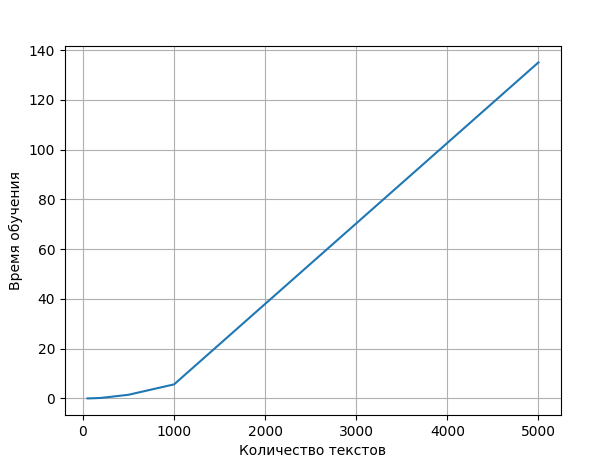
\includegraphics[,scale=0.9]{./img/4.1a.png}
		\caption{График зависимости времени обучения от размера выборки}  
		\label{img:4.1a}
\end{figure}

\captionsetup{justification=centering,singlelinecheck=off}
\begin{figure}[h!]
	\centering
		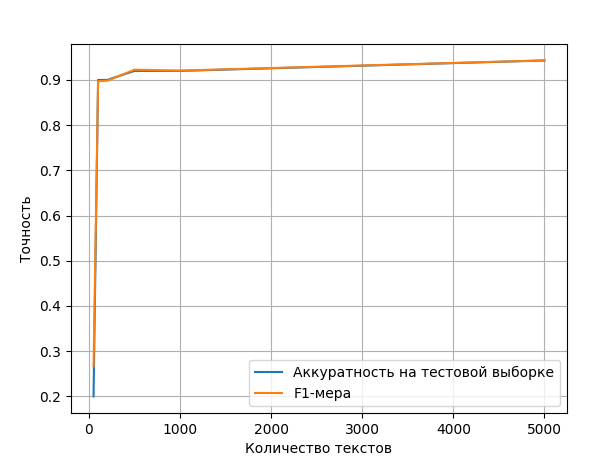
\includegraphics[,scale=0.85]{./img/4.1b.png}
		\caption{График зависимости качества классификатора от размера выборки}  
		\label{img:4.1b}
\end{figure}
\newpage

На основании полученных результатов можно сделать вывод, что количество текстов в обучающей выборке влияет на время обучения и качество классификатора. При использовании выборок с меньшим количеством текста классификатор будет обучаться за меньшее время, но с низкой точностью. По мере увеличения количества текстов в обучающей выборке точность классификатора также увеличивается. Стоит отметить, что увеличение количества текстов увеличивает время обучения, но существенно не увеличивает точность классификатора после того, как количество текстов достигнет 1000.

Таким образом, можно обучить классификатор на выборке из 1000 текстов для оптимизации времени обучения и качества классификатора.

\section{Влияние наличия стоп-слов в тексте}
На этапе предварительной обработки текста происходит процесс удаления стоп-слов. Как отмечалось ранее, стоп-слова --- это текстовые шумы или неинформативные слова, которые встречаются в большом количестве, но не имеют семантического значения и при игнорировании этих слов исходное предложение не теряет своего смысла.

Для проведения данного исследования было проведено сравнение зависимости качества классификатора от наличия процесса удаления стоп-слов на этапе предварительной обработки текстов.

Результаты проведенного исследования приведены в таблице \ref{tab:4.2}.

\begin{table}[H]
	\centering
	\caption{Зависимость качества классификатора от наличия стоп-слов}\label{tab:4.2}
	\begin{tabular}{|m{5em}|m{6.9em}|m{7em}|m{5.5em}|m{4.8em}|}
		\hline
        \textit{Количество текстов} & \textit{Точность на тестовой выборке (Без)} & \textit{Точность на тестовой выборке (С)} & \textit{F1-мера (Без)} & \textit{F1-мера (С)}\\ \hline
		50 & 0.2 & 0.2 & 0.27 &0.27 \\ \hline
        100 & 0.9 & 0.95 & 0.89 &0.94\\ \hline
        200 & 0.9 & 0.90 & 0.90 &0.90\\ \hline
        500 & 0.92 & 0.93 & 0.92 &0.93\\ \hline
        1000 & 0.92 & 0.91 & 0.92 &0.91\\ \hline
        5000 & 0.943 & 0.933 & 0.94 &0.93\\ \hline
	\end{tabular}
\end{table}

Ниже, на рисунках \ref{img:4.2a} и \ref{img:4.2b}, представлены данные из таблицы \ref{tab:4.2} в виде графика.

\captionsetup{justification=centering,singlelinecheck=off}
\begin{figure}[h!]
	\centering
		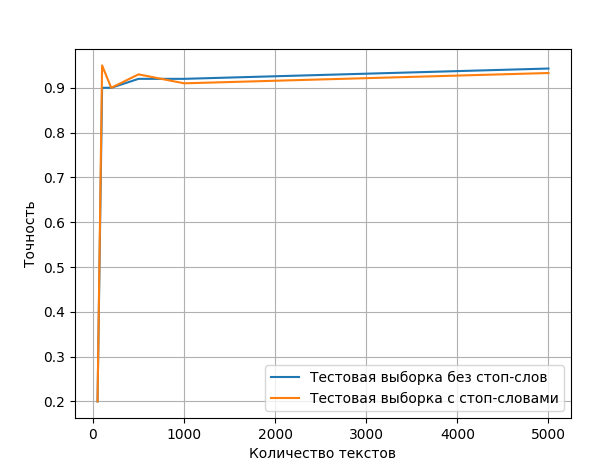
\includegraphics[,scale=0.85]{./img/4.2a.png}
		\caption{График зависимости точности классификатора от наличия стоп-слов}  
		\label{img:4.2a}
\end{figure}

\captionsetup{justification=centering,singlelinecheck=off}
\begin{figure}[h!]
	\centering
		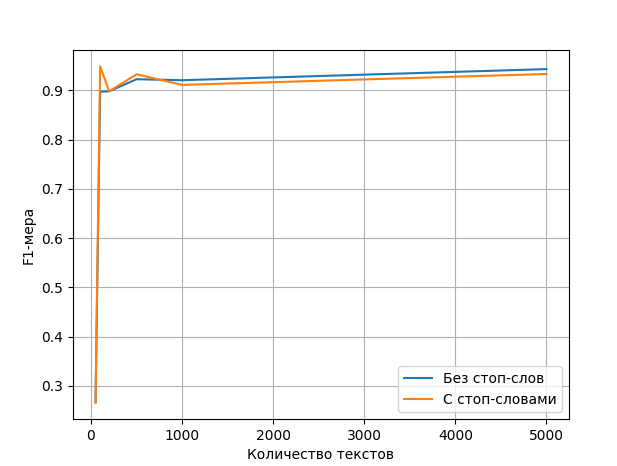
\includegraphics[,scale=0.9]{./img/4.2b.png}
		\caption{График зависимости F1-меры от наличия стоп-слов}  
		\label{img:4.2b}
\end{figure}
\newpage

На основании полученных результатов можно сделать вывод, что наличие стоп-слов в тексте обучающей выборки не сильно влияет на качество классификатора. В обучающих выборках с небольшим количеством текста (с 50 до 500 текстов) с стоп-словами обученные на них классификаторы имеют несколько более высокую точность, чем классификаторы, обученныы на обучающих выборках без стоп-слов (на 1-2\%). Но в обучающих выборках с большим количеством текстов (1000 или 5000 текстов) классификаторы, обученные на обучающих выборках без стоп-слов, имеют более высокую точность (на 1\%).

\section{Влияние ядра метода опорных векторов}
Ядро (kernel) в методе опорных векторов определяет функцию, которая вычисляет скалярное произведение двух векторов в пространстве признаков. Оно позволяет проецировать данные в более высокомерное пространство, где они могут быть линейно разделимыми, даже если исходное пространство не является линейно разделимым. 

Для проведения этого исследования было проведено сравнение зависимости качества классификатора от ядра метода опорных векторов при использовании следующих ядер: линейное, полиномиальное, Гауссово RBF и сигмоидальное.

Ниже, на рисунках \ref{img:4.3a} и \ref{img:4.3b}, представлены результаты проведенного исследования 
\captionsetup{justification=centering,singlelinecheck=off}
\begin{figure}[h!]
	\centering
		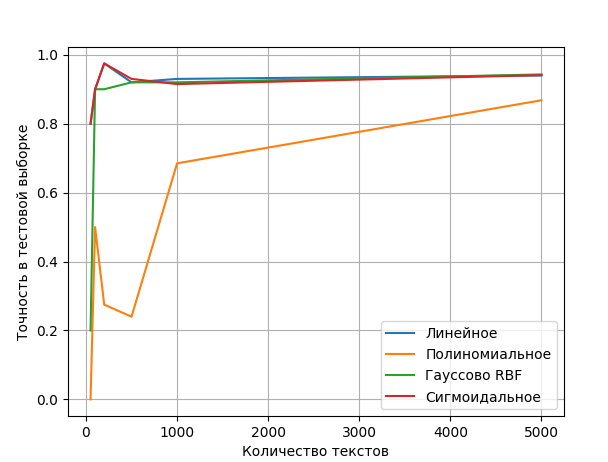
\includegraphics[,scale=0.9]{./img/4.3a.png}
		\caption{График зависимости точности классификатора от ядер}  
		\label{img:4.3a}
\end{figure}

\captionsetup{justification=centering,singlelinecheck=off}
\begin{figure}[h!]
	\centering
		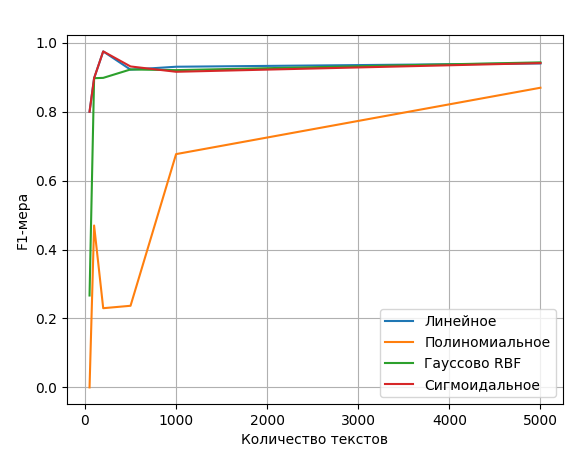
\includegraphics[,scale=0.9]{./img/4.3b.png}
		\caption{График зависимости F1-меры от ядер}  
		\label{img:4.3b}
\end{figure}
\newpage

Из полученных результатов можно сделать вывод, что зависимости точности и F1-меры классификатора от различных ядер совпадают. Классификатор с полиномиальным ядром имеет наименьшее качество, а классификаторы с другими ядрами имеет примерно одинаковую точность.

\section*{Вывод}
В этом разделе были описаны технические характеристики устройства для проведения исследований и приведены исследования разработанного метода. Из полученных результатов исследований можно сделать вывод, что при увеличении количества текстов в обучающей выборке время обучения классификатора будет быстро увеличиваться, но точность классификатора возрастает ненамного для обучающих выборок с большим количеством текстов. Результаты также показывают, что процесс удаления стоп-слов на этапе предварительной обработки текста не сильно влияет на качество классификатора. Использование различных ядер для классификатора показывает, что использование линейного ядра, гауссовского ядра RBF и сигмоидального ядра приводит к получению высокоточного классификатора.

	\part*{ЗАКЛЮЧЕНИЕ}
\addcontentsline{toc}{part}{ЗАКЛЮЧЕНИЕ}
В рамках настоящей работы был разработан, реализован и исследован метод классификации новостных текстов по тематикам с использованием опорных векторов. Все поставленные задачи были выполнены.

Был проведен анализ предметной области. Были рассмотрены методы очистки и предварительной обработки текста. Был проведен обзор методов извлечения признаков из текста.

Был рассмотрены и проанализированы основные методы классификации текстов. Была представлена формализованная постановка задачи в виде IDEF0-диаграммы.

Были описаны этапы работы алгоритма разрабатываемого метода, также были рассмотрены функциональные схемы обучения классификатора и метод классификации. 

Были приведены метрики, используемые для оценки качества работы обученного классификатора. Был описан используемый набор данных для обучения классификатора и была рассмотрена структура программного обеспечения.

Были приведены выбор языка программирования и средства программирования и рассмотрены необходимые библиотеки, которые используются для разработки программного обеспечения. Также был описан формат входных и выходных данных. Также были приведены описание пользовательского интерфейса и руководство пользователя для установки и использования программного обеспечения.

Были описаны технические характеристики устройства для проведения исследований и приведены исследования разработанного метода

Для реализованного метода можно предложить следующие развития:
\begin{itemize}[label = ---]
    \item ускорение работы метода.
    \item добавление возможности работы с различными языками.
\end{itemize}


	% \addcontentsline{toc}{part}{СПИСОК ИСПОЛЬЗОВАННЫХ ИСТОЧНИКОВ}
\renewcommand\bibname{СПИСОК ИСПОЛЬЗОВАННЫХ ИСТОЧНИКОВ}
% \bibliography{biblio}
% \bibliographystyle{utf8gost780u}

    \printbibliography[title=\centerline{СПИСОК ИСПОЛЬЗОВАННЫХ ИСТОЧНИКОВ}]
	\addcontentsline{toc}{part}{\textbf{СПИСОК ИСПОЛЬЗОВАННЫХ ИСТОЧНИКОВ}}
	\chapter*{\centerline{ПРИЛОЖЕНИЕ А}}
\addcontentsline{toc}{part}{\textbf{ПРИЛОЖЕНИЕ А}}
\centering Презентация
	% \chapter*{\centerline{ПРИЛОЖЕНИЕ Б}}
\addcontentsline{toc}{part}{\textbf{ПРИЛОЖЕНИЕ Б}}

\subsection*{Модуль работы с изображениями}
	% \chapter*{\centerline{ПРИЛОЖЕНИЕ В}}
\addcontentsline{toc}{part}{\textbf{ПРИЛОЖЕНИЕ В}}
\end{document}